\documentclass[a4paper,11pt]{jsarticle}


% 数式
\usepackage{amsmath,amsfonts,amssymb}
\usepackage{bm}
% 画像
\usepackage[dvipdfmx]{graphicx}
\usepackage{siunitx}
\usepackage{wrapfig}
\usepackage{cases}
\usepackage{dcolumn}
\makeatletter
\newcommand{\figcaption}[1]{\def\@captype{figure}\caption{#1}}
\newcommand{\tblcaption}[1]{\def\@captype{table}\caption{#1}}
\makeatother

\usepackage{listings,jvlisting}
\lstset{
basicstyle={\ttfamily},
identifierstyle={\small},
commentstyle={\smallitshape},
keywordstyle={\small\bfseries},
ndkeywordstyle={\small},
stringstyle={\small\ttfamily},
frame={tb},
breaklines=true,
columns=[l]{fullflexible},
numbers=left,
xrightmargin=0zw,
xleftmargin=3zw,
numberstyle={\scriptsize},
stepnumber=1,
numbersep=1zw,
lineskip=-0.5ex
}

\begin{document}

\title{スクアット動作の関数化}
\author{平林}
\date{\today}
\maketitle

\begin{figure}[h]
  \centering
  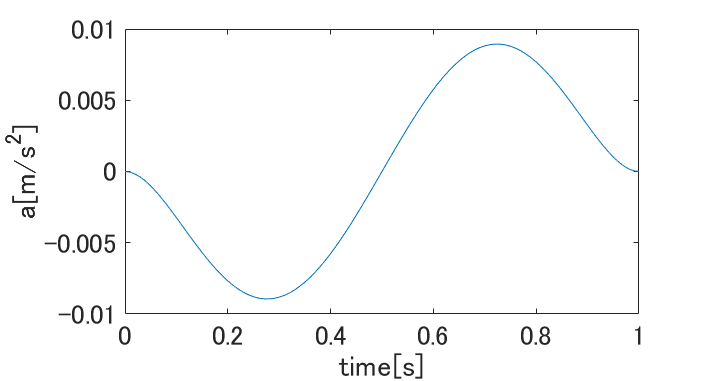
\includegraphics[width = 1\textwidth]{acceleration.png}
  \caption{加速度}
  \label{fig:acceleration}
\end{figure}
しゃがみ込む時の加速度は図\ref{fig:acceleration}のよう。
この関数は
\begin{align*}
  a(t) = t^2{\left(t-1\right)}^2\left(t-\frac{1}{2}\right).
\end{align*}
これを積分して
\begin{align*}
  v(t) &= \frac{t^6}{6}-\frac{t^5}{2}+\frac{t^4}{2}-\frac{t^3}{6} \\
  x(t) &= \frac{t^7}{42}-\frac{t^6}{12}+\frac{t^5}{10}-\frac{t^4}{24}
\end{align*}
グラフは図\ref{fig:velocity},\ref{fig:position}のようになる。
\begin{figure}[h]
  \begin{tabular}{cc}
    \begin{minipage}[t]{0.5\textwidth}
      \centering
      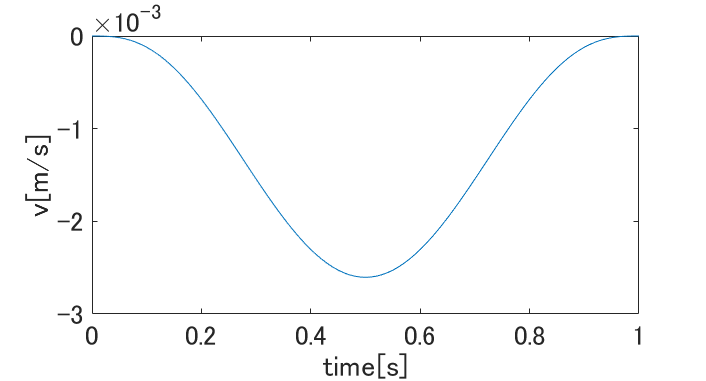
\includegraphics[width = 1\textwidth]{velocity.png}
      \caption{速度}
      \label{fig:velocity}
    \end{minipage} &
    \begin{minipage}[t]{0.5\textwidth}
      \centering
      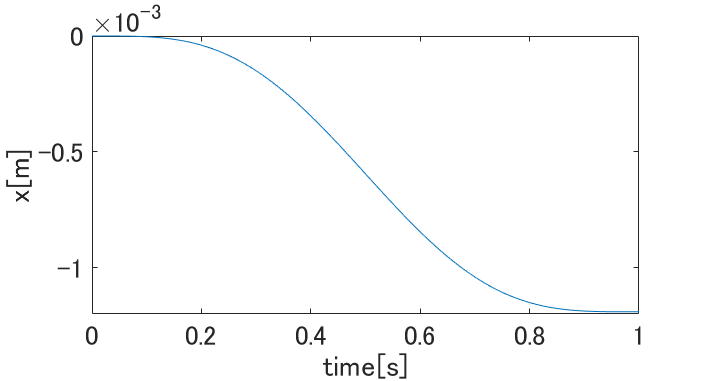
\includegraphics[width = 1\textwidth]{position.png}
      \caption{位置}
      \label{fig:position}
    \end{minipage}
  \end{tabular}
\end{figure}
% \begin{figure}[h]
%   \centering
%   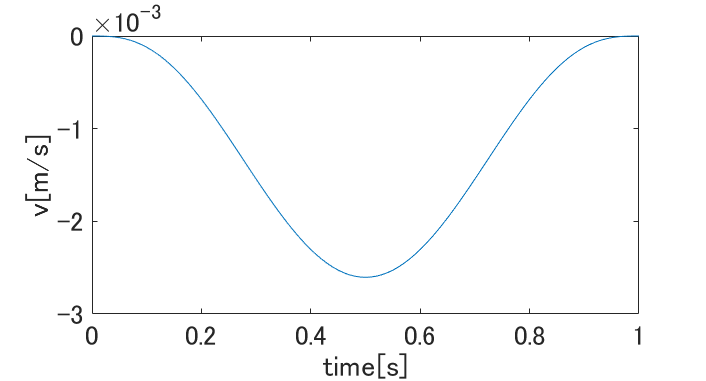
\includegraphics[width = 1\textwidth]{velocity.png}
%   \caption{速度}
%   \label{fig:velocity}
% \end{figure}
% \begin{figure}[h]
%   \centering
%   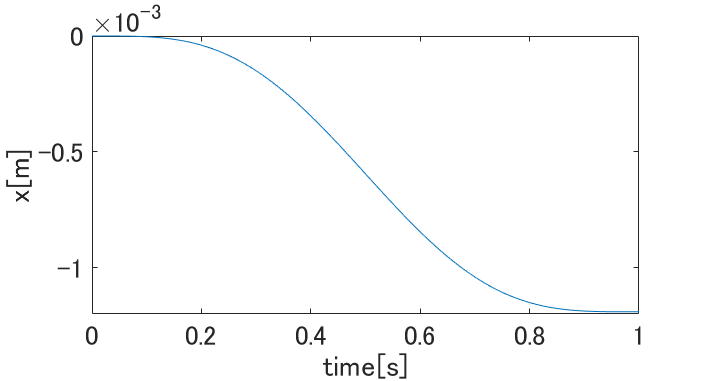
\includegraphics[width = 1\textwidth]{position.png}
%   \caption{位置}
%   \label{fig:position}
% \end{figure}

ただし
\begin{align*}
  x(1) = -\frac{1}{840}
\end{align*}
となるので、$a, v, x$すべて840倍した方が奇麗かもしれない。

\end{document}